\documentclass{scrartcl}

% importations de packages utiles
\usepackage[backend=biber, style=alphabetic]{biblatex}
\addbibresource{rng.bib}
\usepackage[utf8]{inputenc}  % pouvoir écrire avec des accents
\usepackage[french]{babel}  % francophopnie
\usepackage{amsmath, amssymb}
\usepackage{hyperref}  % liens clicables dans pdf final
\usepackage{tikz}  % pouvoir tracer des dessins sympas
\usepackage{listingsutf8}  % rendu de "code" (avec config ci-dessous)
\definecolor{lstcolor}{rgb}{0.9,0.95,0.95}
\definecolor{lstcommentcolor}{rgb}{0.,0.2,0.}
\lstset{
  frameround=tttt,
  %autogobble,
  frame=single,
  backgroundcolor=\color{lstcolor},
  % extendedchars=true,
  % basicstyle=\ttfamily\small,
  keywordstyle=\bfseries\color{blue},
  identifierstyle=\bfseries\color{red},
  stringstyle=\bfseries\color{orange},
  commentstyle=\color{lstcommentcolor},
  language=Python,
  keepspaces=True,
  basicstyle=\fontfamily{pcr}\selectfont\small, % monospace it for copypasting
  upquote=true,
  columns=flexible,
  showstringspaces=False,
  literate={é}{{\'e}}1
}
\title{Générateurs de nombres aléatoires}
\subtitle{Algorithmes et Structures de Données II, GymInf}
\author{Juan-Carlos Barros, Yves Dethurens, Daniel Kessler et Jean-Francis Ravoux}
% et c'est parti
\begin{document}
\maketitle

\tableofcontents

\section{Introduction}

Un générateur de nombres aléatoires (random number generator - RNG) est sensé
produire une suite de nombres respectant une certaine distribution probabiliste,
qui peut être discrète (figure \ref{fig:discdistr}) ou continue (figure 2).

\begin{figure}[h]
  \centering
  \begin{tabular}{cc}
    \begin{tikzpicture}[scale=.6, every node/.style={scale=0.5}]
      \draw[->] (-.2,0) -- (5.5,0) node[right] {$x$};
      \draw[->] (0, -0.2) -- (0, 4.2) node[above] {$f(x)$};
      \foreach \i in {1, ..., 5} {
        \draw[blue] (\i, 0) -- (\i, 3.5);
        \node at (\i, -0.3) {$\i$};
        }
      \draw (.1, 3.5) -- (-.1, 3.5) node[left] {$0.2$};
    \end{tikzpicture}&
      \begin{tikzpicture}[scale=.6, every node/.style={scale=0.5}]
        \draw[->] (-1.2,0) -- (5.2,0) node[right] {$x$};
        \draw[->] (-1,-0.2) -- (-1,6.2) node[above] {$f(x)$};
        \draw[blue] (0, 0) -- (0, 1);
        \draw[blue] (1, 0) -- (1, 4);
        \draw[blue] (2, 0) -- (2, 6);
        \draw[blue] (3, 0) -- (3, 4);
        \draw[blue] (4, 0) -- (4, 1);
        \foreach \i in {0, ..., 5} {
          \node[below] at (\i, 0) {$\i$};
          }
      \end{tikzpicture}
    \\
    {uniforme} & {binômiale}
  \end{tabular}\par
  $f(x)$ est la probabilité de tirer $x$, avec $f(x)\geq0, \;\forall x$ et
  $\sum_xf(x)=1$
  \caption{Distibutions discrètes}
  \label{fig:discdistr}
\end{figure}
\begin{figure}[h]
  \centering

  \begin{tikzpicture}
    \draw[->] (-.2,0) -- (4.2,0) node[right] {$x$};
    \draw[->] (0,-0.2) -- (0,2.2) node[above] {$f(x)$};
    \draw[blue] (1, 0) -- (1, 1) -- (3, 1) -- (3, 0);
    \draw (1, .1) -- (1, -.1) node[below] {\small$c$};
    \draw (3, .1) -- (3, -.1) node[below] {\small$d$};
    \node at (2, 2.2) {uniforme};
    \def\dx{6.8}; \def\dy{-3};
    \draw[->] (-4.2+\dx, \dy) -- (4.2+\dx,\dy) node[right] {$x$};
    \draw[->] (\dx-1,\dy-.2) -- (\dx-1, 2.2+\dy) node[above] {$f(x)$};
    \draw[blue] (\dx, \dy) plot[domain=-4:4, samples=200] ({\x+\dx},{\dy+2*2^(-\x*\x)});
    \draw (\dx, .1+\dy) -- (\dx, \dy-.1) node[below] {\small$\mu$};
    \def\ec{1.3}
    \draw (\dx+\ec, .1+\dy) -- (\dx+\ec, \dy-.1) node[below] {\small$\mu+\sigma$};
    \draw (\dx-\ec, .1+\dy) -- (\dx-\ec, \dy-.1) node[below] {\small$\mu-\sigma$};
    \node at (\dx+1, \dy+2.3) {normale};
    \def\dx{8}; \def\dy{.5};
    \draw[->] (\dx-.2, \dy) -- (\dx+3.2,\dy) node[right] {$x$};
    \draw[->] (\dx-.1,\dy-.2) -- (\dx-.1, \dy+2.2) node[above] {$f(x)$};
    \node[blue] at (\dx+1.5, \dy+1) {\Huge ?};
    \node at (\dx+1.5, \dy+2.2) {autre};
  \end{tikzpicture}
\par
  $\int_a^bf(x)dx$ est la probabilité de tirer $x$ entre $a$ et $b$,
  avec $f(x)\geq0,\forall x$ et $\int_{-\infty}^{+\infty}f(x)dx=1$

  \caption{Distibutions continues}
  \label{fig:contdistr}
\end{figure}

Dans un article datant des années 1950, Von Neumann\cite{VonNeumann} pose les
deux questions fondamentales concernant la génération de nombres aléatoires:
\begin{enumerate}
\item Comment peut-on produire une séquence de chiffres aléatoires? (il est
  question de chiffres décimaux entre 0 et 9, mais la question est la même pour
  des bits 0 ou 1)
\item Comment peut-on produire des nombres réels répartis suivant une loi de
  distribution donnée?
\end{enumerate}
Pour la deuxième question, la réponse existe déjà à ce moment-là: en partant
d'une distribution uniforme entre 0 et 1 (obtenue par exemple à partir d'une
suite de bits aléatoires $(0.b_1b_2b_3\ldots)_{bin}$), en utilisant la fonction
inverse de la distribution cumulée, ont peut reproduire n'importe quelle
distribution continue. En effet, pour une distribution $f:I\rightarrow[0,1]$
donnée, où $I$ est un intervalle où $f$ est strictement positive, la
distribution cumulée correspondante $c:x\mapsto\int_{-\infty}^xf(\xi)d\xi$ est
bijective de $I$ vers l'intervalle $[0,1]$. Son inverse $c^{(-1)}$ permettra
donc de retrouver des valeurs de $x$ distribuées selon $f$. Des méthodes plus
efficaces existent pour des distributions particulières.\par\medskip



Pour la première question, deux approches sont possibles: partir d'un processus
physique, ou bien utiliser une méthode arithmétique. Von Neumann considère que
le hasard idéal sera trouvé dans des phénomènes nucléaires, dont on peut compter
la parité en un laps de temps donné (par exemple: pair:0, impair:1), mais
d'autres moyens plus abordables existent, comme nous le verrons dans la section
\ref{s:TRNG}.

Selon Von Neumann, ``\textit{anyone who considers arithmetical methods of
  producing random digits is, of course, in a state of sin}''.  Cependant, même
s'il était praticable d'utiliser toujours une méthode ``physique'', les méthodes
arithmétiques ont le grand avantage d'être reproductibles: ``\textit{the real
  objection to this procedure is the practical need for checking
  computations}''.
\par\medskip

De nos jours, la considération de reproductibilité de suites aléatoires pour
tester des algorithmes et méthodes numériques comportant une composante
aléatoire demeure tout autant vraie. A contrario, lorsque des nombres aléatoires
sont employés pour la cryptographie, on veut éviter le plus possible la
reproductibilité. Dans ce dernier cas, on préfère autant que possible recourir
exclusivement à la génération de ``vrais'' nombres aléatoires (True Random
Number Generators ou TRNG, section \ref{s:TRNG}). Cependant, ceux-ci sont
coûteux en temps. C'est pourquoi dans tous les autres cas, on utilisera des
méthodes arithmétiques pseudo-aléatoires (Pseudo-Random Number Generators ou
PRNG) produisant de manière déterministe une suite de nombres uniformément
distribués (section \ref{s:PRNG}).
\par\medskip

Finalement, Von Neumann nous met en garde sur le fait que dans les méthodes
arithmétiques grossières qui étaient employées aux années 1950, une bonne part
du ``pseudo-hasard'' provenait en réalité des erreurs d'arrondi, qui sont en
l'occurrence très difficiles à étudier et donc diminuent la prédictibilité de la
distribution des nombres produits. Des méthodes plus modernes devraient éviter
cet écueil.


\section{Générateurs de suites pseudo-aléatoires}\label{s:PRNG}

\subsection{Exemple ``naïf''}
Une méthode utilisée au début des années 1950 consistait simplement à prendre le
carré d'un nombre et le tronquer, comme dans l'exemple suivant:
\[
  30472901 \overset{\text{carré}}\longrightarrow {\color{blue}0928}59769535{\color{blue}5801}
  \overset{\text{tronqué}}\longrightarrow 59769535
\]

Avec, dans l'exemple, un nombre à 8 chiffres au départ, on arrive à un nombre à
16 chiffres après élever au carré (peut-être avec un 0 initial), mais on ne
garde que les 8 chiffres du milieu. On peut bien sûr faire exactement la même
chose avec des nombres en écriture binaire avec par exemple 32 bits au début et
à la fin et 64 à l'étape intermédiaire.

\subsection{Caractéristiques communes}
En gardant dans la tête l'exemple précédent, on peut déjà dégager des
caractéristiques importantes des PRNG.
\subsubsection{la \textit{seed}}
Les suites de nombres pseudo-aléatoires fournissent une manière déterministe de
passer d'un nombre à un autre, sans histoire (seul le nombre précédent est pris
en compte). Cependant, il faut démarrer la suite avec un premier nombre: la
\textit{seed}. Celle-ci pourra être obtenue par une méthode de ``vrai'' hasard
(cf. section \ref{s:TRNG}) ou bien être imposée de manière à pouvoir reporduire
une séquence pseudo-aléatoire donnée, par exemple à des fins de tests.
\subsubsection{la période}
Toutes les séquences pseudo-aléatoires sont en fait périodiques. Si par exemple
on produit des nombres constitués de 32 bits, au maximum au bout de $2^{32}$
itérations on retombera sur la ``seed'' choisie au départ. Dans l'idéal, on ne
voudrait pas y retomber avant. Une bonne méthode de génération de nombres
pseudo-aléatoires devra donc garantis une période longue.

\subsection{Les générateurs linéaires congruents (LCG)}
Le générateur à congruence linéaire est un générateur de nombres aléatoires qui
a été mis au point en 1949 par Derrick Lehmer. Elle est basée sur une fonction
linéaire et l'arithmétique modulaire. Cela en fait une méthode déterministe dont
la période dépend dans une large part de ses paramètres.  Le caractère
déterministe a pour intérêt la reproductibilité des résultats permettant d'une
part la recherche d'erreur dans les codes et d'autre part comme référence pour
des résultats scientifiques.  Une suite $(X_n)$ de nombres est produite par
itération à partir d'une graine: $X_{n+1} = (a X_n +c)[m]$ Où $[m]$ est le
module $m$, $a$ le multiplicateur, $c$ l'incrément et $X_0$ la graine.

La division entière dans la formule permet d'obtenir le reste de la division
entière. Ainsi, à partir de la graine, chaque nombre peut être un entier entre 0
et $m-1$.  Par conséquent, dans le meilleur des cas, $m$ nombres sont produits
et la suite se répète.  Un enjeu est donc de choisir un module suffisamment
grand de sorte d'avoir une suite de nombres longue.

\subsection{Choix des paramètres}
La conjugaison des paramètres $a$, $c$ et $m$ est donc décisive dans le
caractère aléatoire de la suite générée. Ceci est illustré sur des exemples
simples:

1er cas:\par
$X_{n+1} = (3 X_n +2)[5]$ avec $X_0 = 1$ donne pour suite $[1,0,2,3,1,..]$ et la
période est de 4.  2ème cas:\par
$X_{n+1} = (4 X_n +2)[9]$ avec $X_0 = 4$ donnant $[4,0,2,1,6,8,7,3,5,4]$ avec
une période de 9 qui est maximale.  Ainsi, le choix des paramètres obéit à des
critères qui rendent maximale la période dénommés usuellement "magic numbers".
D'autre part, on a pu remarque dans le premier cas que le nombre 4 est absent de
la liste. S'il avait été donné comme graine, la période aurait été de 1 avec
uniquement pour sortie la valeur 4.

En conclusion, la combinaison de paramètres permet une grande variété de
résultats mais ne doit pas occulter l'importance de la graine pour obtenir des
nombres les plus aléatoires possibles.

\subsection{Des générateurs à congruence linéaire types}
Il existe un spectre important de générateurs utilisés dans tous les
langages. Citons en particulier les cas suivants: Fonction RANDU d'IBM :
$X_{n+1} =65539 X_{n} [2^{31}]$\par
Turbo Pascal : $X_{n+1} =(129 X_{n} + 907633385)[2^{32}]$\par
Fonction \texttt{rand()} (C ANSI) :
$X_{n+1} =(1103515245 X_{n}+12345) [2^{31}]$\par
où le module est de l'ordre de 32 bits à la limite maximale des ordinateurs
utilisés.

\subsection{Tests de validité}
Afin de tester la validité des du générateur on peut effectuer un \textit{ test
  spectral}. Celui-ci permet d'observer directement la corrélation de la suite
de nombres.  Il s'agit de représenter les nombres les uns en fonction des autres
dans un espace multidimensionnel de façon à identifier les redondances.  Le
générateur $X_{n+1} =(7 X_{n})[101]$ donnent un histogramme des 101 premiers
nombres avec la graine $X_0 = 1$ sur la figure ci-dessous à gauche:
\begin{figure}
  \begin{center}
    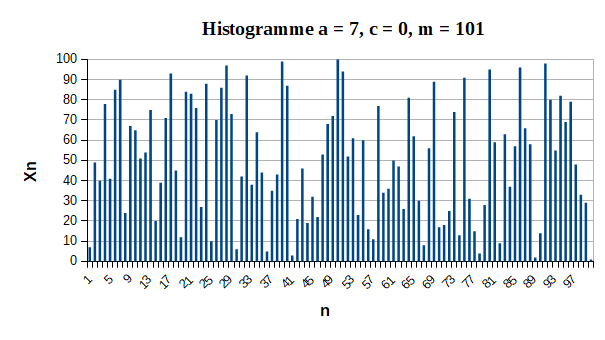
\includegraphics[scale=0.4]{img/histo7Xn[101].png}
    \hspace{0.1\textwidth}
    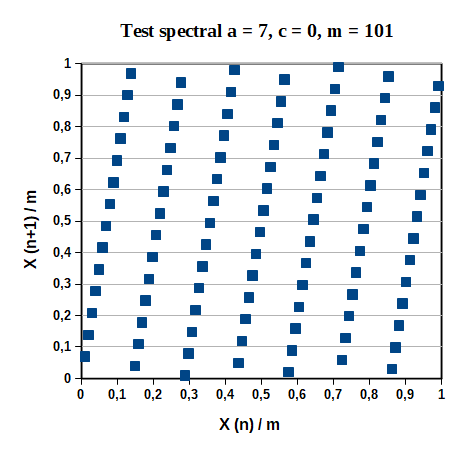
\includegraphics[scale=0.4]{img/a7m101.png}
  \end{center}
\end{figure}
Cet histogramme montre la présence de toutes les valeurs possibles sans période
inférieure à la valeur du module.  Afin de mettre en évidence les corrélations,
on trace les 101 premières paires consécutives de nombres
($X_n/m$,$X_{n+1}/m$). Chaque nombre est normalisé par le module permettant de
visualiser dans l'espace $[0,1]^2$.  Sur la figure de droite, on y constate le
recouvrement des valeurs entre 0 et 1. Le caractère déterministe apparaît avec
les points à distance régulière suivent des droites. De plus, plus cette
distance est faible plus le recouvrement est important.

\subsection{Mersenne Twister et les LFSR}\label{s:MT}
La méthode la plus employée de nos jours est en fait le \textbf{Mersenne
  Twister} \cite{MT}. Une de ses particularités est de garder en mémoire à
chaque étape non pas 1 mais 624 nombres de 32 bits. Chaque itération est un
\textit{twist} de ces 624 nombres, dont les variations permettent d'atteindre
une période de $2^{19937}-1$ (qui est un nombre de Mersenne, d'où le nom du
procédé). Si on n'utilise que le premier des 624 nombres à chaque itération, on
verra que le nombre considéré peut être parfois répété (mais l'état global des
624 nombres aura changé).

L'algorithme du Mersenne Twister est assez compliqué et hors de la portée de ce
travail. Notons cependant qu'il se base sur les  \textbf{Linear-Feedback Shift
  Register}, une classe d'algorithmes dont un autre représentant, le
\textbf{xorshift}, est aussi employé pour la génération de nombres
pseudo-aléatoires. Il est pour l'instant moins courrant mais plus efficace que
le Mersenne Twister.\footnote{https://en.wikipedia.org/wiki/Xorshift}

\subsection{Vrai chaos déterministe}
\subsubsection{Pseudo-aléatoire avec suites chaotiques?x}
Le problème des générateurs basés sur la théorie des nombres, c’est qu’ils
produisent des séquences périodiques, qui possèdent des propriétés qui rend la
suite en partie prévisible, parce que les nombres générés sont dépendants de
ceux qui les précèdent, ce qui ne se produit jamais dans une vraie suite
aléatoire ! \par
D’autres générateurs, basés sur la théorie du chaos, sont imprévisibles (par
définition, voir plus bas), mais il est généralement plus difficile de garantir
que ceux-ci ont une période longue, et ils sont moins répandus que les
générateurs basés sur la théorie des nombres. \par
Le générateur de nombres pseudo-aléatoires présenté ci-dessous (Saito \&
Yamaguchi \cite{SY}) utilise les deux théories pour produire des suites qui
ressemblent à de vraies suites aléatoires non périodiques. Son coût
computationnel est élevé, mais les séquences générées peuvent par exemple servir
de référence pour des tests qualitatifs.

\subsubsection{Point de départ: le décalage de Bernouilli}
La relation $\alpha_{n+1}=(2\alpha_n)\ mod\ 1$ définit une suite où
$\alpha_n \in [0;1[$. En arrondissant les termes de cette suite, on obtient une
séquence binaire pseudo-aléatoire. \par
Exemple : $\alpha_0$ = 0.3 donne la suite \{ 0.3; \textbf{0.6}; 0.2; 0.4; 0.8;
\textbf{0.6}; … \} \par
ou la séquence 01001100110011001... qui est périodique et donc très
prévisible. \par
Mais si $\alpha_0$ est \textbf{irrationnel}, cette suite devient \textbf{non
  périodique}. Cela signifie qu’une infinitésimale variation de $\alpha_0$
provoquera un changement radical à un moment de la séquence. Cette forte
sensibilité aux conditions initiales est une caractéristique des fonctions
chaotiques : au bout d'un certain temps, un phénomène chaotique devient
imprévisible.  Une loi déterministe va évidemment être prévisible si ses
paramètres sont entièrement connus. Mais si les conditions initiales contiennent
une part d’incertitude (par exemple une imprécision, même minime), alors un tel
processus chaotique ne permet plus de prévision à long terme.

\begin{table}
\begin{tabular}{|*{7}{c|}}
& \multicolumn{3}{|c|}{suite irrationnelle} 
& \multicolumn{3}{|c|}{suite rationnelle} \\
$n$ & $\alpha_n$ & valeur & $\epsilon_n$ & $\overline{\epsilon}_n$ & valeur & $\overline{\alpha}_n$ \\ 
\hline
0 & $\pi/4$ & \textbf{0.78539816} & 1 & 1 & \textbf{0.78539823} & $\frac{355}{452}$ \\
1 & $\pi/2-1$ & 0.57079632 & 1 & 1 & 0.57079646 & $\frac{258}{452}$ \\
2 & $\pi-3$ & 0.14159265 & 0 & 0 & 0.14159292 & $\frac{64}{452}$ \\
3 & $2\pi-6$ & 0.28318530 & 0 & 0 & 0.28318584 & $\frac{128}{452}$ \\
4 & 4$\pi$‒12 & 0.56637061 & 1 & 1 & 0.56637168 & $\frac{256}{452}$ \\
5 & 8$\pi$‒25 & 0.13274122 & 0 & 0 & 0.13274336 & $\frac{60}{452}$ \\
6 & 16$\pi$‒50 & 0.26548245 & 0 & 0 & 0.26548672 & $\frac{120}{452}$ \\
7 & 32$\pi$‒100 & 0.53096491 & 1 & 1 & 0.53097345 & $\frac{240}{452}$ \\
8 & 64$\pi$‒201 & 0.06192982 & 0 & 0 & 0.06194690 & $\frac{28}{452}$ \\
9 & 128$\pi$‒402 & 0.12385965 & 0 & 0 & 0.12389380 & $\frac{56}{452}$ \\
10 & 256$\pi$‒804 & 0.24771931 & 0 & 0 & 0.24778761 & $\frac{112}{452}$ \\
11 & 512$\pi$‒1608 & 0.49543863 & 0 & 0 & 0.49557522 & $\frac{224}{452}$ \\
12 & 1024$\pi$‒3216 & 0.99087727 & 1 & 1 & 0.99115044 & $\frac{448}{452}$ \\
13 & 2048$\pi$‒6433 & 0.98175455 & 1 & 1 & 0.98230088 & $\frac{444}{452}$ \\
14 & 4096$\pi$‒12867 & 0.96350910 & 1 & 1 & 0.96460176 & $\frac{436}{452}$ \\
15 & 8192$\pi$‒25735 & 0.92701820 & 1 & 1 & 0.92920353 & $\frac{420}{452}$ \\
16 & 16384$\pi$‒51471 & 0.85403641 & 1 & 1 & 0.85840707 & $\frac{388}{452}$ \\
17 & 32768$\pi$‒102943 & 0.70807283 & 1 & 1 & 0.71681415 & $\frac{324}{452}$ \\
18 & 65536$\pi$‒205887 & 0.41614566 & 0 & 0 & 0.43362831 & $\frac{196}{452}$ \\
19 & 131072$\pi$‒411774 & 0.83229132 & 1 & 1 & 0.86725663 & $\frac{392}{452}$ \\
20 & 262144$\pi$‒823549 & 0.66458264 & 1 & 1 & 0.73451327 & $\frac{332}{452}$ \\
21 & 524288$\pi$‒1647099 & 0.32916528 & 0 & 0 & 0.46902654 & $\frac{212}{452}$ \\
22 & 1048576$\pi$‒3294198 & 0.65833057 & 1 & 1 & 0.93805309 & $\frac{424}{452}$ \\
23 & 2097152$\pi$‒6588397 & 0.31666114 & 0 & 1 & 0.87610619 & $\frac{396}{452}$ \\
23 & 4194304$\pi$‒13176794 & 0.63332228 & 1 & 1 & 0.75221238 & $\frac{340}{452}$ \\
24 & 8388608$\pi$‒26353589 & 0.26664456 & 0 & 1 & 0.50442477 & $\frac{228}{452}$ \\
25 & 16777216$\pi$‒52707178 & 0.53328913 & 1 & 0 & 0.00884955 & $\frac{4}{452}$ \\
26 & 33554432$\pi$‒105414357 & 0.06657826 & 0 & 0 & 0.01769911 & $\frac{8}{452}$ \\
27 & 67108864$\pi$‒210828714 & 0.13315653 & 0 & 0 & 0.03539823 & $\frac{16}{452}$ \\
28 & 134217728$\pi$‒421657428 & 0.26631307 & 0 & 0 & 0.07079646 & $\frac{32}{452}$ \\
29 & 268435456$\pi$‒843314856 & 0.53262615 & 1 & 0 & 0.14159292 & $\frac{64}{452}$ \\
\end{tabular}
\caption{Exemple comparé, avec $\alpha_0 = \frac{\pi}{4}$ et
  $\overline{\alpha}_0 = \frac{355}{452}$, deux valeurs très proches
  \label{t:chaos}
}
\end{table}

\subsubsection{Sensibilité aux conditions initiales}
On voit (cf. Table \ref{t:chaos}) que les deux suites, malgré un point de départ
presque identique, divergent complètement à partir de n = 20. Cela montre le
caractère chaotique de la structure : sans la connaissance de la huitième
décimale de $\alpha_0$, impossible de prévoir le comportement de cette suite
au-delà du 20e terme.\par
On sait dès lors que l’observation des 20 premiers termes ne permet pas d’en
déduire la suite.\par
\par
\textbf{Problème} : si on s’intéresse à la suite irrationnelle, parfaitement
aléatoire en apparence, le problème est qu’il faut connaître le nombre
irrationnel de départ (ici $\alpha_0 = \frac{\pi}{4}$) avec une précision
croissante. Cela demandera un temps de calcul de plus en plus important, et ne
ne sera plus possible pour de très grandes valeurs de $n$. \par
Il faut pouvoir gérer des valeurs exactes pour $\alpha_n$!

\subsubsection{Racines irrationnelles du 3e degré}
Saito et Yamaguchi \cite{SY} proposent une solution à ce problème: en
choisissant $\alpha_0$ comme racine d’un polynôme du 3e degré $f_0$ dont les
coefficients sont entiers, et qui a une unique racine réelle. \par
Ainsi, on peut facilement déterminer le polynôme $f_1$ dont $\alpha_1$ est la
racine, et ainsi de suite. \par
Exemple : on pose $f_0(x) = x^3+x–1$ et $f_n(x) = x^3+b_nx^2+c_nx–d_n$, avec
$f_n(\alpha_n) = 0$, et $\epsilon_n = (\alpha_n)$.
\begin{center}
  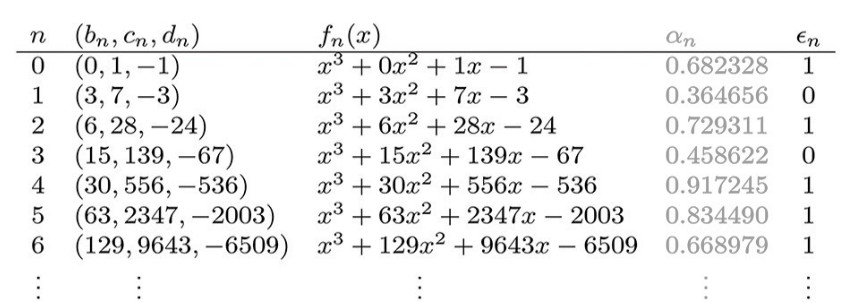
\includegraphics[scale=0.75]{img/SaitoYamaguchi2017.png}  
\end{center}

\subsubsection{Calcul de la séquence}
Alors les relations ci-dessous permettent d'éviter le calcul des $\alpha_n$:\par
\begin{tabular}{ l l }
  $a_n$ = 1 & $b_{n+1}$ = $2b_n+3\epsilon_n$ \\
  $c_{n+1} = 4c_n+(4b_n+3)\epsilon_n$ 
            & $d_{n+1} = 8d_n+(4c_n+2b_n+1)\epsilon_n$ \\
  \multicolumn{2}{l}{$1 + 2b_n + 4c_n + 8d_n < 0 \ \Leftrightarrow \ \alpha_n > \frac{1}{2} \ \Leftrightarrow \ \epsilon_n = 1 $}
\end{tabular}\par
La production de la séquence pseudo-aléatoire
$\{\epsilon_n\}_{n \in \mathbb{N}}$ consiste donc à déterminer les termes de la
suite $\{ (b_n,c_n,d_n,\epsilon_n) \}_{n \in \mathbb{N}}$. Celle-ci se construit
entièrement avec des opérations élémentaires, sans avoir à extraire les racines
$\alpha_n$ qui restent implicites. \par
\medskip Selon les auteurs, en choisissant bien les coefficients du polynôme
initial $f_0$, on peut vérifier que la séquence binaire produite est presque
uniformément distribuée sur l’intervalle [0;1]. \par


\section{Comment générer de ``vrais'' nombres aléatoires?}\label{s:TRNG}
\subsection{De la bonne graine...}
Les algorithmes qu'on a vus permettent de générer des suites de nombres pseudo aléatoires, c'est à dire qu'on ne peut pas distinguer d'une suite réellement aléatoire. Ceci dit, il y a un gros problème avec ces algorithmes: ils sont tous déterministes et cela entraîne la nécessité de trouver une graine imprévisible car si on peut deviner la graine, on découvre toute la suite de nombres aléatoires générée!\par
Comment générer cette bonne graine?

\subsection{Source d'entropie interne}
Une source de hasard peut être trouvée au coeur de l'ordinateur. Il existe en effet des algorithmes qui combinent de nombreuses sources d'entropie dans l’état interne de l’ordinateur pour en tirer un résultat proche du vrai aléatoire. \par
On peut citer, par exemple, HAVEGE (HArdware Volatile Entropy Gathering and Expansion) qui est implémenté dans le noyau Linux pour créer des graines utilisables par les algorithmes PRNG.\par
HAVEGE combine des milliers de paramètres de l’état interne (horloge, registres du CPU, mémoire cache, branch predictor, mouvements de souris, etc) puis en tire un nombre qui est très proche d'un vrai aléatoire; il est en tous cas impossible à deviner car il dépend de trop nombreux paramètres qu’un hackeur ne pourrait pas geler ou découvrir en temps réel.
Pour plus de détails: voir \href{https://www.irisa.fr/caps/projects/hipsor/misc.php}{ici}.

\subsection{Source d'entropie externe}
On l'a dit, l'ordinateur est incapable de produire du hasard pur. Par contre, le monde physique, lui, regorge d'entropie: on est toujours embêté par l’incertitude des mesures et par le fait qu’on ne peut pas contrôler une grandeur physique avec une précision arbitraire. \par
Il semble donc que le monde physique pourrait nous fournir une vraie source aléatoire. \par
On va voir deux catégories de sources physiques:
\begin{itemize}
\item phénomènes classiques (statistiques)
\item phénomènes quantiques (individuels)
\end{itemize}

\subsubsection{Entropie classique}
Parmis les sources d’entropie naturelle, on trouve tous les processus stochastiques où des lois microscopiques (déterministes ou pas) régissent l'évolution de nombreuses particules; ceci aboutit à une mesure macroscopique (comme la température) qu’il est impossible de prédire avec une précision infinie car elle dépend de trop de paramètres (état interne). \par
Un exemple typique est le bruit thermique correspondant aux fluctuations de la tension électrique aux bornes d’une résistance à une certaine température. En effet, le mouvement imprévisible des électrons se traduit en courant électrique et ceci affecte la tension. \par
Ceci a été découvert en 1927 par Johnson puis expliqué théoriquement par Nyquist (\href{https://journals.aps.org/pr/abstract/10.1103/PhysRev.32.97}{Johnson} \& \href{https://journals.aps.org/pr/abstract/10.1103/PhysRev.32.110}{Nyquist}). \par
Imaginons donc qu’on mesure la variation de la tension aux bornes de la résistance, on aurait une bonne source de hasard. \par
Un autre exemple serait la mesure de la hauteur de l'eau dans un océan. La houle ou les vagues provoquées par le vent entraînent là aussi une impossibilité de prévoir à long terme la hauteur de l'eau. Il convient de remarquer que l'échantillonage des valeurs aléatoires ne devra pas dépasser une certaine fréquence qui dépend de la source employée. En effet, si on prend la hauteur de l'eau chaque seconde, par exemple, les mesures seront fortement corrélées alors que si on mesure une fois par heure, il sera impossible de trouver une corrélations entre les mesures.\par
Mais même si la suite temporelle de valeurs de la tension ou de la hauteur de l'eau est chaotique, elle n'est pas forcément entièrement imprévisible, dumoins en théorie. C'est ce que mettent en avant les défenseurs de la prochaine source d'entropie...

\subsubsection{Entropie quantique}
Les phénomènes quantiques ont l’avantage d’être intrinsèquement indéterministes. 
Exemples: 
\begin{itemize}
\item source radioactive détectée par un compteur Geiger (imaginé par Von Neumann)
\item photons traversant un miroir semi-réfléchissant
\end{itemize}
Dans ces deux cas, on ne peut pas deviner le résultat d’une mesure, même si l'on connaît parfaitement l’état interne du système car il est dans une superposition quantique d’états que seule la mesure va briser en \href{https://fr.wikipedia.org/wiki/R\%C3\%A9duction_du_paquet_d\%27onde}{réduisant le paquet d’onde}.
On va décrire un peu plus en détails la deuxième car elle est très utilisée actuellement, notamment par l'entreprise ID Quantique, leader dans le domaine des QRNG (TRNG quantiques).

\subsubsection{ID Quantique et ses photons}
ID Quantique est une entreprise genevoise, spin off de l’université de Genève, fondée en 2001 par 3 scientifiques (Nicolas Gisin, Hugo Zbinden et l’actuel CEO Grégoire Ribordy qui nous a accordé une interview) \par
Elle a trois principales branches d’activité (\href{https://www.idquantique.com/quantum-sensing/overview/}{détecteurs quantiques}, partage de clefs quantique \href{https://www.idquantique.com/quantum-safe-security/overview/}{QKD} et Génération quantique de nombres aléatoires \href{https://www.idquantique.com/random-number-generation/overview/}{QRNG}) \par
Le principe du QRNG chez ID Quantique est le suivant:
\begin{center}
  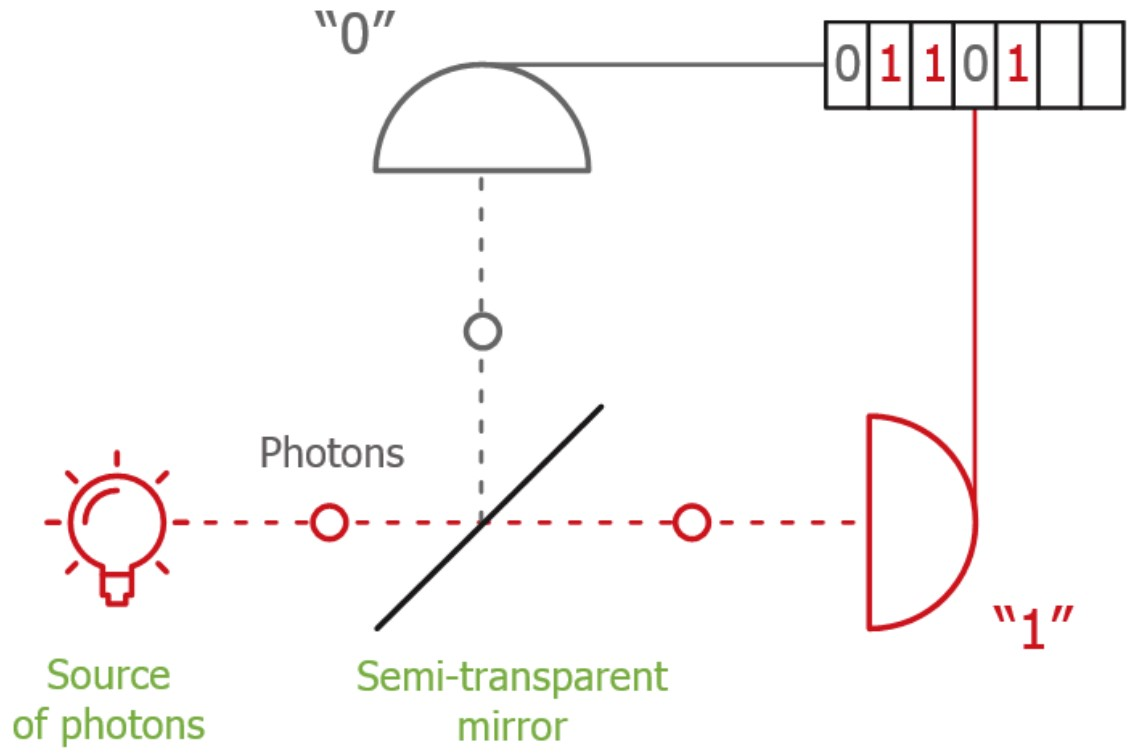
\includegraphics[scale=0.25]{img/Figure1.OpticalSystemUsedTuGenerateRandomNumbers.jpg}  
\end{center}

\begin{enumerate}
\item Une diode LASER émet régulièrement un photon.
\item Le photon émis arrive sur une paroi semi-réfléchissante
\item Deux détecteurs sont à l'affût pour signaler si le photon a traversé ou a été réfléchi par le miroir.
\item Le résultat selon le détecteur atteint produit un “1” ou un “0”.
\item Un traitement logiciel (\href{https://nvlpubs.nist.gov/nistpubs/Legacy/SP/nistspecialpublication800-90r.pdf}{NIST 800-90}, \href{https://content.iospress.com/download/computability/com001?id=computability\%2Fcom001}{anti-aliasing}, etc.) est appliqué à la suite de bits produits pour assurer l’équiprobabilité.
\item Si le débit de nombres aléatoires n’est pas suffisant, on peut utiliser des PRNG se basant sur les graines produites par le QRNG pour l’augmenter.
\end{enumerate}
\begin{center}
  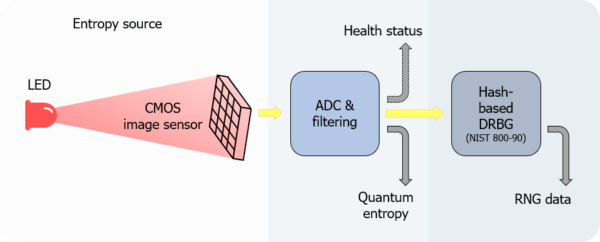
\includegraphics[scale=0.5]{img/QRNG-core-technology-600x242.png}  
\end{center}

Ce processus est fondamentalement imprédictible car au moment où le photon sort de la diode LASER, il n’a aucune caractéristique qui le prédétermine à être plutôt transmis que réfléchi ou l’inverse. En effet, tous les photons sont exactement dans le même état quantique à la sortie d'un LASER. Même au moment où il atteint le miroir, on ne sait toujours pas s’il a traversé ou s’il a été réfléchi car les deux phénomènes se produisent en réalité en parallèle. Ce n’est qu’au moment d’être effectivement détecté dans un des deux chemins que le paquet d’onde est réduit et que le photon devient une “particule réfléchie” ou une “particule transmise”. Impossible donc de recueillir des données innombrables sur l’état interne pour déduire de possibles résultats (comme ce pourrait être envisagé dans un TRNG classique)!


\section{Que fait le module ``random'' de Python?}
Python fait appel à l'OS pour générer des ``vrais'' nombres aléatoires.
Celui-ci implémente typiquement un algorithme HAVEGE.
On peut y accéder directement à travers la classe \texttt{random.SystemRandom} ou par
le module dédié  \texttt{secrets}, qui, comme son nom l'indique, a pour but de
fournir des nombres suffisamment aléatoires pour la cryptographie.

En guise de PRNG, le module \texttt{random} fait appel au Mersenne Twister (voir
section \ref{s:MT}), implémenté de manière sous-jacente en C afin d'être rapide,
efficace et isolé (vu comme une ``opération atomique'' par l'interprétateur
Python, ce qui évite des soucis dans le cadre de la programmation concurrente).
La \textit{seed} par défaut est obtenue par le générateur aléatoire de l'OS,
mais elle peut aussi être initialisée ``à la main'' si nécessaire.

Le module \texttt{random} fournit des fonctions transformant directement les
nombres générés par le Mersenne Twister de manière à émuler plusieurs
distributions aléatoires usuelles (uniforme, normale, etc.) ainsi que le tirage
d'une sous-collection aléatoire d'une collection donnée.
\begin{lstlisting}
  import random

  # entier aléatoire entre 0 et 9
  n = random.randrange(10)

  # flottant aléatoire entre 0 et 10
  x = random.uniform(0, 10)

  # tirage de 2 éléments au hasard d'une liste
  l = random.sample(["a", "b", "c", "d", "e"], 2)
\end{lstlisting}

Un simple test avec des tirages aléatoires en utilisant
\texttt{random.uniform(0, 1)} à partir d'une même seed avec des nombre de
tirages cumulés différents permet d'observer graphiquement comment on se
rapproche d'une distribution uniforme au fur et à mesure que l'on augmente le
nombre de tirages.
\begin{center}
  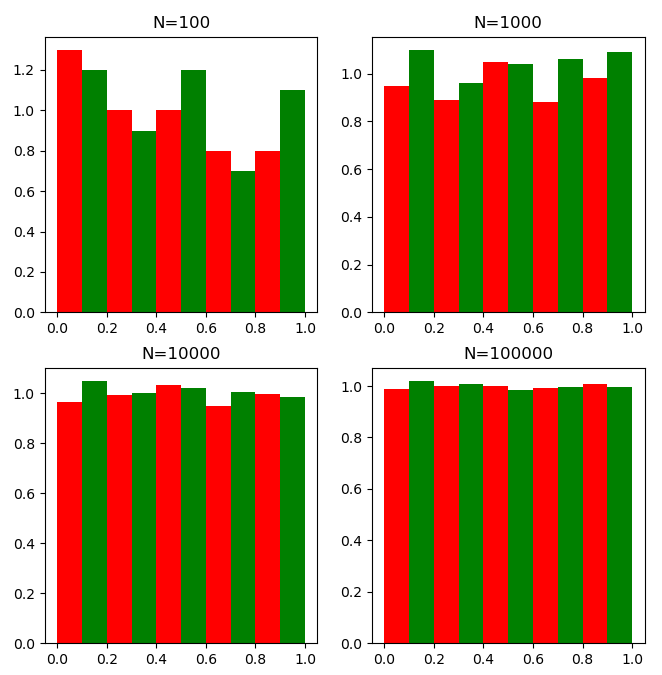
\includegraphics[width=0.8\textwidth]{img/uniformes.png}\par
  (pour le code source: voir le dossier \texttt{Code} dans
  \url{github.com/dalker/ASD2_RNG/})
\end{center}
Nous n'avons pas fait de tests statistiques plus poussés là-dessus, mais il
pourrait être intéressant de vérifier par exemple jusqu'à quel point la fonction
\texttt{random.gaussian()} fournit une distribution proche de la distribution
normale.

\section{Conclusion}
Le sujet de la génération de nombres aléatoires par un ordinateur s'est avéré
beaucoup plus vaste qu'on aurait pu l'imaginer. D'un côté, les méthodes
arithmétiques employant des suites de nombres déterministes de grande période
présentant une distribution quasi-uniforme sont en évolution permanente. De
l'autre, la cryptographie nécessite sans cesse des progrès dans les moyens de
construire des ``vrais'' nombres aléatoires à partir de sources
physiques. Vraisemblablement, il y aura de quoi donner du fil à retordre à
beaucoup de chercheurs pendant les prochaines décennies.

\addcontentsline{toc}{section}{Références}
\printbibliography
\end{document}